\begin{center}
{{\Large \sc High-Performance Computing}}
\end{center}
\rule{\textwidth}{1pt}
\begin{description}
\item[Student name and id:] Marie Mørk \{s112770\} Anja Liljedahl Christensen\{s162876\}
 Andreas Vedel Jantzen \{s162858\}
 Anders Launer Bæk \{s160159\}
\item[Hold name:] matmult\_MAAA
\item[Hand-in:] Matrix Multiplication
\end{description}
\rule{\textwidth}{1pt}


\section{Summary}
Different functions, performing matrix-matrix multiplication are implemented in C in order to compare performance. Cases considered are ordering of the nested loops, optimizers in the compiler and blocking. The implemented functions are compared with the CBLAS subroutine DGEMM. As memory in C is stored row-wise, it has been found that the most optimal ordering of nested loops is to have the column index in the most inner loop. The optimizers are found to enhance performance significantly. The blocked version is found to be less efficient than the optimized version of the most efficient ordering of the loops. This might be due to the implementation of the blocking in which as many columns as rows are considered at a time. 

\section{Statement of the problem}

The goal of the assignment is to create a library of functions that perform matrix-matrix multiplications. Performance of the implementations are to be compared with the DGEMM matrix-matrix multiplication routine from the BLAS library. As input, each of the functions should take the dimensions of the matrices (M, N, K) as well as the matrices (A, B, C), according to figure \ref{fig:matmult}. The problem is divided into four sub-problems; 
\begin{itemize}
    \item Wrap the call DGEMM into a function called \texttt{matmult\_lib()}, that takes the same inputs as
    specified above.
    \item Implement a function that performs double precision matrix-matrix multiplication. The function should be named \texttt{matmult\_nat()}.
    \item Functions for each of the permutations of the three nested loops needed to perform matrix multiplications. The performance of the permutations should be compared. Furthermore, the timings should be compared with and without different compiler optimizations. The functions should be named as \texttt{matmult\_per()}, where \texttt{per} is the ordering of the nested loops for the given implementation, e.g. \texttt{nmk,knm}, ect.
    \item A blocked version of the matrix-matrix multiplication function named \texttt{matmult\_blk()}. This function should take an extra input, \texttt{bs}, which specifies the blocking size.
\end{itemize}

\begin{figure}[h]
    \centering
    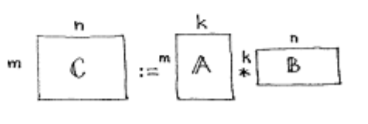
\includegraphics[]{contents/pics_1/matmult.PNG}
    \caption{Visualisation of the matrix-matrix multiplications to be performed. The picture is taken from the problem description on DTU Inside.}
    \label{fig:matmult}
\end{figure}

\section{Hardware and software}\label{sec:hard}

Specifications of the test environment are listed below:
\begin{itemize}
\item CPU information
\begin{itemize}
\item Vendor ID:             GenuineIntel
\item CPU family:            6
\item Model:                 79
\item Model name:            Intel(R) Xeon(R) CPU E5-2650 v4 @ 2.20GHz
\item CPU MHz:               1297.656
\item L1 (d / i) cache:             32K
\item L2 cache:              256K
\item L3 cache:              30720K
\end{itemize}
\item Compiler and Matrix implementations
\begin{itemize}
\item The GCC compiler have been applied with and without compiler optimization using the compiler flag \texttt{-Ofast}. 
\item The library function uses DGEMM from the CBLAS interface
\item Matrices are indexed in the following way: [m] [n]
\item The following line has been specified in the job script: "\texttt{\#BSUB -n 1}" to make sure the batch job only uses one core.
\end{itemize}
\end{itemize}


\section{Theory}
Matrix multiplications are central operations in many numerical algorithms. Due to this, it is essential to make the operation fast to keep the computation time low. In order to achieve an optimal matrix-matrix multiplication algorithm, it is therefore important to take the ordering of nested loops and memory storage in the computer into account.\\


In C matrices are stored row-wise. Hence, when an element is fetched from memory the next couple of elements in the same row are collected as well, since they are stored in the same cache line. This is useful if the next couple of elements from the same row are needed in the near future, since they have already been loaded into memory. If on the other hand the next element is extracted from another row, e.g. in the case of looping through a column, there will be a cache miss and a new cache line is loaded into memory. Thus, in the worst case there will be a cache miss each time a new element is needed. In the case of matrix multiplication it is necessary to loop through both rows and columns in multiple nested loops and hence there is a great chance of cache miss when the matrices are sufficiently large. If the matrices are small enough such that all three will fit in memory there should be no cache misses. For large scale matrices it is essential to optimize the implementation of the matrix-matrix multiplication in order to avoid too many cache misses.\\

Double precision matrix multiplication of square matrices requires space for $3\cdot d^3$ doubles in memory, if the dimensions of the matrices is given by $d$. As storage of a double takes up 8 bits, the maximum dimensions for the matrices to fit in the memory of a given cache is found theoretically by calculating
\begin{align*}
    d = \sqrt{\frac{L/8}{3}}
\end{align*}
where L is the memory in the given cache. The maximum dimensions of square matrices fitting into each of the caches used are listed in table \ref{tab:cache_max_dim}. In reality, the maximum allowed dimensions might be higher, as the program performs hardware prefetch. 
\begin{table}[h]
    \centering
    \begin{tabular}{c|c|c}
         Cache & Size [bytes] & Maximum dimension of Matrix  \\ \hline
         $L_1$ & 32K & 36 \\
         $L_2$ & 256K & 103 \\
         $L_3$ & 30720K & 1131 
    \end{tabular}
    \caption{Maximum dimensions of square matrices fitting into each of the caches.}
    \label{tab:cache_max_dim}
\end{table}

In the last sub problem of the report, blocking is implemented in order to optimize the memory usage in the algorithm. The idea behind blocking is to divide the iterations into smaller blocks, so that operations can be performed for parts of the matrices at a time, instead of considering the full size of the problem. This is especially useful when handling large problems, for which the memory needed to compute the full operation exceeds the bounds of the memory. When using an algorithm that relies on blocking it is important to use one of the respective compiler flags: \texttt{-O3} or \texttt{-Ofast}. By doing so the compiler analyses the code several lines ahead and is hereby able to optimize the code. 
%Notet med optimizers i compileren

%Noget med blocking (evt. sammen med hukommelse) 

% hardware prefetch

%Hit/miss og mflops/s - memory 

\section{Algorithms}
\subsection{\texttt{matmult\_lib}} %Wrapping of GDEMM
The subroutine DGEMM from the library BLAS will be used to evaluate the performance of and compare with the different implementations of the matrix-matrix multiplication. For this purpose the CBLAS interface is used and wrapped into the function \texttt{matmult\_lib} such that the library implementation of the matrix-matrix multiplication takes the same arguments as the other functions.  The call to DGEMM using the CBLAS interface is \texttt{cblas\_dgemm} which takes 14 arguments\footnote{http://www.netlib.org/lapack/explore-html/dc/d18/cblas} as shown in algorithm \ref{alg:lib}. From the inputs, the matrix multiplication is calculated as
\begin{align*}
    C = \alpha \cdot A \cdot B + \beta \cdot C.
\end{align*}
Here, $\alpha$ and $\beta$ are arguments to be specified in the input. In this case $\alpha$ is set to 1 while $\beta$ is set to 0 in order to get the wanted output. The other inputs in DGEMM (aside from M, N, K, A, B, and C) are the layout (set to rowmajor), whether the A and B matrices should be transposed (TRANSA and TRANSB) and the leading dimensions of A, B and C. As seen in the algorithm \ref{alg:lib}, the A and B matrices are not transposed, and the dimensions are set to K, N and N for A, B and C. 
\lstinputlisting[label={alg:lib},caption={\texttt{matmult\_lib}},style=CStyle]{code/matmult_lib.c}

\subsection{\texttt{matmult\_nat}} %nat
The implementation of the \texttt{matmult\_nat} function is listed in algorithm \ref{alg:nat}. For this function, it has been chosen to use the a MNK ordering of the nested loops. That is that the outer loop iterates over the dimension M, the second over N and the inner over K. 
\lstinputlisting[label={alg:nat},caption={\texttt{matmult\_nat}},style=CStyle]{code/matmult_nat.c}

\subsection{\texttt{matmult\_per}} % permutations
The \texttt{matmult\_per} permutations are implemented as presented in algorithm \ref{alg:per}, where the ordering of the nested loops are interchanged for each permutation of M, N and K. There exist six different permutations of the \texttt{matmult\_nat} function, namely MNK, NKM, MKN, KMN, MNK, and NMK. The \texttt{matmult\_per} algorithm has been optimized in relation to the \texttt{matmult\_nat} function. This has been done using stripmining, and setting all entries of C to zero using 1 for loop instead of 2 enables the compiler to perform vectorization.
\lstinputlisting[label={alg:per},caption={\texttt{matmult\_per} for the \texttt{mnk} ordering of the loops.},style=CStyle]{code/permutationcodepiece.c}

\subsection{\texttt{matmult\_blk}} % Blocking
In order to implement blocking in the matrix-matrix multiplications, additional nested loops are needed. The algorithm used for blocking is based on one of the best performing versions of the \texttt{matmult\_per} functions – in this case \texttt{matmult\_mkn}. In algorithm \ref{alg:blk} the function is presented. As mentioned in the problem description \texttt{matmult\_blk} takes the additional input \texttt{bs}, which is the blocking size. In blocking, the matrices A, B and C are portioned into smaller matrices for which the multiplications are performed and then added to each other to get the full C matrix. In this implementation the blocks are chosen to be square matrices. This can be seen from the first three nested loops in which blocks of the matrices of size bs$\times$bs are chosen. In the inner three nested loops the extracted matrices are multiplied and added to C. When using \texttt{matmult\_blk} the compiler needs an optimizer flag, in order for the blocking to set in. 
\lstinputlisting[label={alg:blk},caption={\texttt{matmult\_blk}},style=CStyle]{code/matmult_blk.c}





\newpage
\section{Results}
The implementation of the different functions were checked in a test-script to see if the C matrix was calculated as expected. Each of the functions \texttt{matmult\_nat}, \texttt{matmult\_per}, \texttt{matmult\_blk}, and \texttt{matmult\_lib} were tested using the square matrices:
\begin{align*}
    A_s = 
    \begin{pmatrix}
        1 & 2\\
        2 & 4
    \end{pmatrix} \qquad
    B_s =
    \begin{pmatrix}
        2 & 2\\
        2 & 2
    \end{pmatrix}
\end{align*}
and the non-square matrices:
\begin{align*}
    A_{ns} = 
    \begin{pmatrix}
        1 & 2\\
        2 & 4\\
        3 & 6
    \end{pmatrix} \qquad
    B_{ns} =
    \begin{pmatrix}
        2 & 2 & 2\\
        2 & 2 & 2
    \end{pmatrix}
\end{align*}
which all returned
\begin{align*}
    C_{s} = 
    \begin{pmatrix}
        6 & 6\\
        12 & 12
    \end{pmatrix} \qquad
    C_{ns} = 
    \begin{pmatrix}
        6 & 6 & 6\\
        12 & 12 & 12\\
        18 & 18 & 18
    \end{pmatrix}
\end{align*}
% The calculations are checked against the DGEMM subroutine to ensure that the matrix-matrix multiplication is computed correctly for each of the implemented functions. 
The calculation check sum provided by the driver has also been studied during the performance evaluation of the implemented functions, and in each of the cases the return value was 0 as expected.  

Only square matrices are considered, e.g. N = M = K when the performance of the functions is evaluated. 

Furthermore the performances of the above functions have been evaluated with and without the compiler flag \texttt{-Ofast} which enable compiler optimization, indicated as "opt".
It has been decided to capture the hit and miss counters for the L1 cache and L2 cache in the first project.

\subsection{Performance of \texttt{matmult\_nat}}

Figure \ref{fig:nat_perf} illustrates two realizations of the naive implementation of the \texttt{matmult\_nat} function. The blue realization is the naive implementation without compiler optimization enabled and the black realization has compiler optimization enabled. By considering the differences between the realizations in figure \ref{fig:nat_perf} huge increases in performance can be achieved by using compiler optimization.\\

\begin{figure}[!th]
\centering
\begin{tikzpicture}[scale = 1]
\begin{axis}[
width=17cm, height=8cm,     % size of the image
grid = major,
grid style={dashed, gray!30},
xmode=log,log basis x=10,
xmin=0,    % start the diagram at this
ymin=50,    % start the diagram at this 
ymax=2000, % end   the diagram at this 
axis background/.style={fill=white},
ylabel=Mflops/s,
xlabel=Memory/kbytes]

\addplot[mark=*, blue] table [x=mem, y=mflops, col sep=comma]{data/matmult_nat.txt};
\addlegendentry{matmult\_nat}
\addplot[mark=*, black] table [x=mem, y=mflops, col sep=comma]{data/matmult_nat_opt.txt};
\addlegendentry{matmult\_nat\_opt}


\addplot[red] table [x=x, y=y, col sep=comma]{data/L1.txt};
\addplot[red] table [x=x, y=y, col sep=comma]{data/L2.txt};
\addplot[red] table [x=x, y=y, col sep=comma]{data/L3.txt};
\addlegendentry{L1, L2 and L3 cache}
\end{axis} 
\end{tikzpicture}
\caption{Performance of the \texttt{matmult\_nat} function measured in Mflops/s as a function of kbytes.}
\label{fig:nat_perf}
\end{figure}


Table \ref{tab:L1L2hitmis_nat} reports the cache hits and cache miss for the \texttt{matmult\_nat} function. It is observed that there are fewer hits in the optimized version for the L1 cache, while the misses are of equal size. The hypothesis would be that the number of hits increases for the optimized version, but it might be that the optimizer reduces the memory to be fetched, why the number of hits drops. Even though the number of hits reduces, we can still conclude that the optimized function performs significantly better than the non-optimized.

\begin{table}[!th]
\centering
\begin{tabular}{l|rr|rr|rr|rr}
\multirow{3}{*}{} & \multicolumn{4}{|c}{Non-optimized}& \multicolumn{4}{|c}{Optimized}\\
& \multicolumn{2}{|c}{L1 in $\%$} & \multicolumn{2}{|c}{L2 in $\%$}& \multicolumn{2}{|c}{L1 in $\%$} & \multicolumn{2}{|c}{L2 in $\%$} \\
& Hit& Miss& Hit& Miss& Hit& Miss& Hit& Miss\\ \hline
\texttt{matmult\_nat(50x50)}& 10 & 0 & 0 & 0 &0 & 0 & 0 & 0\\
\texttt{matmult\_nat(850x850)} & 129129 & 6072 & 5368 & 704 & 11651 & 6069 & 5524 & 544\\
\texttt{matmult\_nat(1600x1600)}& 861503 & 34583 & 134 & 34445& 73553 & 31510 & 92 & 31416\\
\end{tabular}
\caption{Hits and miss of the L1 and L2 cache for nat, presented in millions}
\label{tab:L1L2hitmis_nat}
\end{table}
\newpage

The naive implementation of the matrix multiplication routine, \texttt{matmult\_nat} is compared to the library subroutine DGEMM, which has been wrapped in \texttt{matmult\lib}. In figure \ref{fig:nat_perf}, the performance of DGEMM is shown with and without optimization in the compiler. Please note, that the axes is different from the one in \ref{fig:nat_perf}.\\
It is seen from the figure that the performance of DGEMM is nearly the same whether or not an optimizer is used in the compiler. This is not surprising, as we expect the library function to be optimized in itself, and the wrapper funciton \texttt{matmult\_lib} only calls the DGEMM subroutine and assigns values to some of the inputs. The performance of the library sub routine is significantly better than that of \texttt{matmult\_nat}. In table \ref{tab:L1L2hitmis_lib}, the hits and miss of the function are shown. All hits and misses are seen to be zero. This might be a consequence of the way the analyzer function handles the wrapper function. We would have expected the library function to have a very high number of hits and only few misses.

\begin{figure}[!th]
\centering
\begin{tikzpicture}[scale = 1]
\begin{axis}[
width=17cm, height=8cm,     % size of the image
grid = major,
grid style={dashed, gray!30},
xmode=log,log basis x=10,
%xmin=0,    % start the diagram at this
%ymin=50,    % start the diagram at this 
ymax=10000, % end   the diagram at this 
axis background/.style={fill=white},
ylabel=Mflops/s,
xlabel=Memory/kbytes,
legend pos=south east]

%\addplot[mark=*, blue] table [x=mem, y=mflops, col sep=comma]{data/matmult_nat.txt};
%\addlegendentry{matmult\_nat}
\addplot[mark=*, black] table [x=mem, y=mflops, col sep=comma]{data/matmult_lib_opt.txt};
\addlegendentry{matmult\_lib\_opt}

\addplot[mark=*, blue] table [x=mem, y=mflops, col sep=comma]{data/matmult_lib.txt};
\addlegendentry{matmult\_lib}


\addplot[red] table [x=x, y=y, col sep=comma]{data/L1.txt};
\addplot[red] table [x=x, y=y, col sep=comma]{data/L2.txt};
\addplot[red] table [x=x, y=y, col sep=comma]{data/L3.txt};
\addlegendentry{L1, L2 and L3 cache}
\end{axis} 
\end{tikzpicture}
\caption{Performance of the \texttt{matmult\_lib} function measured in Mflops/s as a function of kbytes.}
\label{fig:nat_perf}
\end{figure}

\begin{table}[!th]
\centering
\begin{tabular}{l|rr|rr|rr|rr}
\multirow{3}{*}{} & \multicolumn{4}{|c}{Non-optimized}& \multicolumn{4}{|c}{Optimized}\\
& \multicolumn{2}{|c}{L1 in $\%$} & \multicolumn{2}{|c}{L2 in $\%$}& \multicolumn{2}{|c}{L1 in $\%$} & \multicolumn{2}{|c}{L2 in $\%$} \\
& Hit& Miss& Hit& Miss& Hit& Miss& Hit& Miss\\ \hline
\texttt{matmult\_lib(50x50)}& 0.0 & 0.0 & 0.0 & 0.0&0.0 & 0.0 & 0.0 & 0.0\\
\texttt{matmult\_lib(850x850)}& 0.0 & 0.0 & 0.0 & 0.0 & 0.0 & 0.0 & 0.0 & 0.0\\
\texttt{matmult\_lib(1600x1600)}& 0.0 & 0.0 & 0.0 & 0.0& 0.0 & 0.0 & 0.0 & 0.0\\
\end{tabular}
\caption{Hits and miss of the L1 and L2 cache for lib, presented in millions}
\label{tab:L1L2hitmis_lib}
\end{table}


\newpage
\subsection{Optimal permutations of \texttt{matmult\_nat}}

As mentioned earlier it is possible to create several permutations of the naive \texttt{matmult\_nat} function. The six possible (the naive is included) permutations are presented in figure \ref{fig:opt_nmk_1_non} and the compiler optimized permutations in figure \ref{fig:opt_nmk_1}.


\begin{figure}[!th]
\centering
\begin{tikzpicture}[scale = 1]
\begin{axis}[
width=17cm, height=8cm,     % size of the image
grid = major,
grid style={dashed, gray!30},
xmode=log,log basis x=10,
xmin=0,    % start the diagram at this
ymin=50,    % start the diagram at this 
ymax=400, % end   the diagram at this 
axis background/.style={fill=white},
ylabel=Mflops/s,
xlabel=Memory/kbytes,
legend pos=south west]

\addplot[mark=*, black] table [x=mem, y=mflops, col sep=comma]{data/matmult_nmk.txt};
\addlegendentry{nmk}

\addplot[mark=*, red] table [x=mem, y=mflops, col sep=comma]{data/matmult_nkm.txt};
\addlegendentry{nkm}

\addplot[mark=*, blue] table [x=mem, y=mflops, col sep=comma]{data/matmult_mnk.txt};
\addlegendentry{mnk}



\addplot[mark=*, orange] table [x=mem, y=mflops, col sep=comma]{data/matmult_mkn.txt};
\addlegendentry{mkn}

\addplot[mark=*, green] table [x=mem, y=mflops, col sep=comma]{data/matmult_knm.txt};
\addlegendentry{knm}

\addplot[mark=*, magenta] table [x=mem, y=mflops, col sep=comma]{data/matmult_kmn.txt};
\addlegendentry{kmn}

\addplot[red] table [x=x, y=y, col sep=comma]{data/L1.txt};
\addplot[red] table [x=x, y=y, col sep=comma]{data/L2.txt};
\addplot[red] table [x=x, y=y, col sep=comma]{data/L3.txt};
%\addlegendentry{L1, L2 and L3 cache}
\end{axis} 
\end{tikzpicture}
\caption{Performance of all permutations of the \texttt{matmult\_per} functions measured in Mflops/s as a function of kbytes.}
\label{fig:opt_nmk_1_non}
\end{figure}

\begin{figure}[!th]
\centering
\begin{tikzpicture}[scale = 1]
\begin{axis}[
width=17cm, height=8cm,     % size of the image
grid = major,
grid style={dashed, gray!30},
xmode=log,log basis x=10,
xmin=0,    % start the diagram at this
ymin=0,    % start the diagram at this 
ymax=5000, % end   the diagram at this 
axis background/.style={fill=white},
ylabel=Mflops/s,
xlabel=Memory/kbytes,
legend pos=north west]

\addplot[mark=*, black] table [x=mem, y=mflops, col sep=comma]{data/matmult_nmk_opt.txt};
\addlegendentry{nmk\_opt}

\addplot[mark=*, red] table [x=mem, y=mflops, col sep=comma]{data/matmult_nkm_opt.txt};
\addlegendentry{nkm\_opt}

\addplot[mark=*, blue] table [x=mem, y=mflops, col sep=comma]{data/matmult_mnk_opt.txt};
\addlegendentry{mnk\_opt}



\addplot[mark=*, orange] table [x=mem, y=mflops, col sep=comma]{data/matmult_mkn_opt.txt};
\addlegendentry{mkn\_opt}

\addplot[mark=*, green] table [x=mem, y=mflops, col sep=comma]{data/matmult_knm_opt.txt};
\addlegendentry{knm\_opt}

\addplot[mark=*, magenta] table [x=mem, y=mflops, col sep=comma]{data/matmult_kmn_opt.txt};
\addlegendentry{kmn\_opt}

\addplot[red] table [x=x, y=y, col sep=comma]{data/L1.txt};
\addplot[red] table [x=x, y=y, col sep=comma]{data/L2.txt};
\addplot[red] table [x=x, y=y, col sep=comma]{data/L3.txt};
%\addlegendentry{L1, L2 and L3 cache}
\end{axis} 
\end{tikzpicture}
\caption{Performance of all permutations of the the compiler optimized \texttt{matmult\_***} functions measured in Mflops/s as a function of kbytes.}
\label{fig:opt_nmk_1}
\end{figure}

% \begin{figure}[!th]
% \centering
% \begin{tikzpicture}[scale = 1]
% \begin{axis}[
% width=17cm, height=8cm,     % size of the image
% grid = major,
% grid style={dashed, gray!30},
% xmode=log,log basis x=10,
% xmin=0,    % start the diagram at this
% ymin=0,    % start the diagram at this 
% ymax=5000, % end   the diagram at this 
% axis background/.style={fill=white},
% ylabel=Mflops/s,
% xlabel=Memory/kbytes,
% legend pos=north west]

% \addplot[mark=*, black] table [x=mem, y=mflops, col sep=comma]{data/matmult_mkn_opt.txt};
% \addlegendentry{mkn\_opt}

% \addplot[mark=*, red] table [x=mem, y=mflops, col sep=comma]{data/matmult_knm_opt.txt};
% \addlegendentry{knm\_opt}

% \addplot[mark=*, blue] table [x=mem, y=mflops, col sep=comma]{data/matmult_kmn_opt.txt};
% \addlegendentry{kmn\_opt}

% \addplot[red] table [x=x, y=y, col sep=comma]{data/L1.txt};
% \addplot[red] table [x=x, y=y, col sep=comma]{data/L2.txt};
% \addplot[red] table [x=x, y=y, col sep=comma]{data/L3.txt};
% %\addlegendentry{L1, L2 and L3 cache}
% \end{axis} 
% \end{tikzpicture}
% \caption{Performance of the compiler optimized \texttt{matmult\_mkn}, \texttt{matmult\_knm} and \texttt{matmult\_kmn} functions measured in Mflops/s as a function of kbytes.}
% \label{fig:opt_nmk_2}
% \end{figure}

Figure \ref{fig:opt_nmk_1_non} tells that \texttt{matmult\_mkn} and \texttt{matmult\_kmn} are the best performing permutations in the L3 cache. Hence having N as the last index, makes the matrix-matrix multiplication the fastest. This was also expected, because M and K are the row indexes of the input matrices and fits to the way memory is stored the most efficient way. \\
The permutations has calculated using an optimizer. This result is presented in \ref{fig:opt_nmk_1}. This confirms that \texttt{matmult\_mkn} and \texttt{matmult\_kmn} are the fastest permutations, having \texttt{matmult\_mkn} a bit faster. When the optimizer is used the performance difference already occours in L1 and definately in L2. Hence, the combination of optimizer and having the right indexing makes \texttt{matmult\_mkn} the fastest permutation. \\ 
Table \ref{tab:L1L2hitmis_1600}, \ref{tab:L1L2hitmis_850} and \ref{tab:L1L2hitmis_50} presents the cache hits and misses for L1 and L2.
The functions have been evaluated for 50, 850 and 1600 and the global variable \texttt{} has been set to perform 10 iterations in each loop in order to make comparable tests. Table \ref{tab:L1L2hitmis_850} and \ref{tab:L1L2hitmis_1600} does again confirm that \texttt{matmult\_mkn} and \texttt{matmult\_kmn} are the most optimal matrix-matrix multiplication indexing. This can be concluded because the ratio of their respective hits and misses are big, both for L1 and L2. 

\begin{table}[!th]
\centering
\begin{tabular}{l|rr|rr|rr|rr}
\multirow{3}{*}{50x50} & \multicolumn{4}{|c}{Non-optimized}& \multicolumn{4}{|c}{Optimized}\\
& \multicolumn{2}{|c}{L1} & \multicolumn{2}{|c}{L2}& \multicolumn{2}{|c}{L1} & \multicolumn{2}{|c}{L2} \\
& Hit& Miss& Hit& Miss& Hit& Miss& Hit& Miss\\ \hline
\texttt{matmult\_nmk}& 10 & 0.0 & 0.0 & 0.0 &0 & 0 & 0 & 0\\
\texttt{matmult\_nkm}& 10 & 0.0 & 0.0 & 0.0&0 & 0 & 0 & 0\\
\texttt{matmult\_mnk}& 10 & 0.0 & 0.0 & 0.0 &0 & 0 & 0 & 0 \\
\texttt{matmult\_mkn}& 10 & 0.0 & 0.0 & 0.0&0 & 0 & 0 & 0\\
\texttt{matmult\_knm}& 10 & 0.0 & 0.0 & 0.0&0 & 0 & 0 & 0\\
\texttt{matmult\_kmn}& 10 & 0.0 & 0.0 & 0.0 & 0 & 0 & 0 & 0
\end{tabular}
\caption{Hits and miss of the L1 and L2 cache for 50x50}
\label{tab:L1L2hitmis_50}
\end{table}

\begin{table}[!th]
\centering
\begin{tabular}{l|rr|rr|rr|rr}
\multirow{3}{*}{850x850} & \multicolumn{4}{|c}{Non-optimized}& \multicolumn{4}{|c}{Optimized}\\
& \multicolumn{2}{|c}{L1} & \multicolumn{2}{|c}{L2}& \multicolumn{2}{|c}{L1} & \multicolumn{2}{|c}{L2} \\
& Hit& Miss& Hit& Miss& Hit& Miss& Hit& Miss\\ \hline
\texttt{matmult\_nmk}& 129209 & 6094 & 6081 & 10& 11291 & 6350 & 6338 & 7 \\
\texttt{matmult\_nkm}& 123043 & 12138 & 11430 & 707 &13814 & 13310 & 12714 & 593\\
\texttt{matmult\_mnk}& 129169 & 6072 & 5364 & 703 &11851 & 6024 & 5448 & 573 \\
\texttt{matmult\_mkn}& 135215 & 192 & 16 & 2& 356 & 531 & 528 & 2\\
\texttt{matmult\_knm} & 123043 & 12144 & 11446 & 696& 13693 & 13341 & 12765 & 576 \\
\texttt{matmult\_kmn}& 135215 & 35 & 25 & 90& & 3524 & 525 & 509 & 18
\end{tabular}
\caption{Hits and miss of the L1 and L2 cache for 850x850}
\label{tab:L1L2hitmis_850}
\end{table}

\begin{table}[!th]
\centering
\begin{tabular}{l|rr|rr|rr|rr}
\multirow{3}{*}{1600x1600} & \multicolumn{4}{|c}{Non-optimized}& \multicolumn{4}{|c}{Optimized}\\
& \multicolumn{2}{|c}{L1} & \multicolumn{2}{|c}{L2}& \multicolumn{2}{|c}{L1} & \multicolumn{2}{|c}{L2} \\
& Hit& Miss& Hit& Miss& Hit& Miss& Hit& Miss\\ \hline
\texttt{matmult\_nmk}& 861423 & 34484 & 86 & 34397 & 51572 & 33418 & 26 & 33390 \\
\texttt{matmult\_nkm}& 819981 & 75809 & 121 & 75685 &11379 & 64094 & 134 & 63958\\
\texttt{matmult\_mnk}& 861623 & 34644 & 124 & 34518 &73593 & 31507 & 92 & 31412\\
\texttt{matmult\_mkn}& 901463 & 262 & 2464 & 16 & 22983 & 3790 & 3774 & 17\\
\texttt{matmult\_knm}& 820021 & 75806 & 89 & 75715 & 114034 & 64055 & 118 & 63937\\
\texttt{matmult\_kmn}& 901383 & 211 & 172 & 39 & 22943 & 3627 & 3521 & 105
\end{tabular}
\caption{Hits and miss of the L1 and L2 cache for 1600x1600}
\label{tab:L1L2hitmis_1600}
\end{table}

\newpage




% \todo[inline]{Hvad viser disse nedenstående plots??}
% From the Figure \ref{fig:permatrix}, \ref{fig:perhits} and \ref{fig:permisses} we can tell that the permutations that has N as the last index, is the ones that run the fastest. This makes sense because index K and M is the rows index's of the input matrices. The memory is build the way that it is faster to read rows than columns, which one can make a benefit of when indexing loops the right way. 

% \begin{figure}[!th]
% \centering
% \begin{tikzpicture}[scale = 1]
% \begin{axis}[
% width=17cm, height=8cm,     % size of the image
% grid = major,
% grid style={dashed, gray!30},
% %xmode=log,log basis x=10,
% ymode=log,log basis y=10,
% %xmin=0,    % start the diagram at this x-coordinate
% %xmax=10, % end   the diagram at this x-coordinate
% %ymin=0,    % start the diagram at this y-coordinate
% %ymax=11000, % end   the diagram at this y-coordinate
% %/pgfplots/xtick={0,1,...,10}, % make steps of length 5 
% %/pgfplots/ytick={0,1,...,10}, % make steps of length 5 
% axis background/.style={fill=white},
% xlabel=CPU time [s],
% ylabel=Matrix size,
% legend style={at={(0.03,0.5)},anchor=center}]

% \addplot[mark=*,red] table [x=CPUsec, y=L2Misses, col sep=comma]{data/plotmnk.txt};
% \addlegendentry{matmult\_mnk()}

% \addplot[mark=*,blue] table [x=CPUsec, y=L2Misses, col sep=comma]{data/plotmkn.txt};
% \addlegendentry{matmult\_mkn()}

% \addplot[mark=*,green] table [x=CPUsec, y=L2Misses, col sep=comma]{data/plotnmk.txt};
% \addlegendentry{matmult\_nmk()}

% \addplot[mark=*,black] table [x=CPUsec, y=L2Misses, col sep=comma]{data/plotnkm.txt};
% \addlegendentry{matmult\_nkm()}

% \addplot[mark=*,magenta] table [x=CPUsec, y=L2Misses, col sep=comma]{data/plotkmn.txt};
% \addlegendentry{matmult\_kmn()}

% \addplot[mark=*,yellow] table [x=CPUsec, y=L2Misses, col sep=comma]{data/plotknm.txt};
% \addlegendentry{matmult\_knm()}

% \end{axis} 
% \end{tikzpicture}
% \caption{Misses on permutations}
% \label{fig:permisses}
% \end{figure}











\newpage
\subsection{Blocking version}
As mentioned in the section on algorithms, the blocked version is based on \texttt{matmult\_mkn} because it is the best performing permutation of the \texttt{matmult\_nat} function, see figure \ref{fig:opt_nmk_1_non}. 

Figure \ref{fig:blk_opti} illustrates a realization of the performance of \texttt{matmult\_blk} as a function of \texttt{bs} for $M=N=K=1500$. This problem size has been chosen for the experiment because three matrices of this size only fits in the L3 cache. Seeing as the blocking version performs operations on smaller blocks of the problem at a time, even though the full problem does not fit in the first two caches, the subproblems might fit and hence improve computation time. The red vertical lines in the figure illustrates the theoretical maximum blocking size for the matrices to fit in the memory of cache L1, L2, and L3 respectively. The maximum sizes are calculated in the theory section and are equal to those presented in table \ref{tab:cache_max_dim}.

Close to the boarder of L1, Mflops/s fluctuates a lot which can be caused by the hardware prefetching. Even though it is not visible on the logarithmic scale used for the blocking size, other experiments have shown that the drop in Mflops/s occurs just after the limit of L1. This is due to hardware prefetching and optimization of the compiler. The same behaviour is seen for L2. It is surprising that Mflops/s drops again well before the theoretical L3 limit, as we would have expected the drop to occur closer to the limit. The premature drop might be due to the implementation of blocking.

\begin{figure}[!th]
\centering
\begin{tikzpicture}[scale = 1]
\begin{axis}[
width=17cm, height=8cm,     % size of the image
grid = major,
grid style={dashed, gray!30},
xmode=log,log basis x=10,
%xmin=0,    % start the diagram at this
ymin=1300,    % start the diagram at this 
ymax=1550, % end   the diagram at this 
axis background/.style={fill=white},
ylabel=Mflops/s,
xlabel=block size,
legend pos=south east]

\addplot[mark=*, blue] table [x=mnk, y=mflops, col sep=comma]{data/matmult_blk_1500_bs.txt};
\addlegendentry{bs}

\addplot[red] table [x=x, y=y, col sep=comma]{data/L1_blk.txt};
\addplot[red] table [x=x, y=y, col sep=comma]{data/L2_blk.txt};
\addplot[red] table [x=x, y=y, col sep=comma]{data/L3_blk.txt};
\addlegendentry{L1, L2 and L3 cache}
\end{axis} 
\end{tikzpicture}
\caption{Performance of the \texttt{matmult\_blk} function measured in Mflops/s as a function of block size.}
\label{fig:blk_opti}
\end{figure}
 


\begin{figure}[!th]
\centering
\begin{tikzpicture}[scale = 1]
\begin{axis}[
width=17cm, height=8cm,     % size of the image
grid = major,
grid style={dashed, gray!30},
xmode=log,log basis x=10,
xmin=0,    % start the diagram at this
ymin=800,    % start the diagram at this 
ymax=1700, % end   the diagram at this 
axis background/.style={fill=white},
ylabel=Mflops/s,
xlabel=Memory/kbytes,
legend pos=south east]

\addplot[mark=*, black] table [x=mem, y=mflops, col sep=comma]{data/matmult_blk_36_opt.txt};
\addlegendentry{blk\_36\_opt}
\addplot[mark=*, red] table [x=mem, y=mflops, col sep=comma]{data/matmult_blk_103_opt.txt};
\addlegendentry{blk\_103\_opt}
\addplot[mark=*, blue] table [x=mem, y=mflops, col sep=comma]{data/matmult_blk_1103_opt.txt};
\addlegendentry{blk\_1103\_opt}

\addplot[red] table [x=x, y=y, col sep=comma]{data/L1.txt};
\addplot[red] table [x=x, y=y, col sep=comma]{data/L2.txt};
\addplot[red] table [x=x, y=y, col sep=comma]{data/L3.txt};
%\addlegendentry{L1, L2 and L3 cache}
\end{axis} 
\end{tikzpicture}
\caption{Performance of the \texttt{matmult\_blk\_opt} for different block sizes with compiler optimization.}
\label{fig:opt_blk_1}
\end{figure}

Figure \ref{fig:opt_blk_1} illustrates the three realizations of the  \texttt{matmult\_blk\_opt}. The three realizations illustrates that the choice of block size is depends on the problem size, e.g. the size of the matrix.


\begin{table}[!th]
\centering
\begin{tabular}{l|rr|rr|rr|rr|rr|rr}
\multirow{3}{*}{} & \multicolumn{4}{|c}{bs = 36}& \multicolumn{4}{|c}{bs = 103} & \multicolumn{4}{|c}{bs = 1103}\\
& \multicolumn{2}{|c}{L1 in $\%$} & \multicolumn{2}{|c}{L2 in $\%$}& \multicolumn{2}{|c}{L1 in $\%$} & \multicolumn{2}{|c}{L2 in $\%$}& \multicolumn{2}{|c}{L1 in $\%$} & \multicolumn{2}{|c}{L2 in $\%$} \\
& Hit& Miss& Hit& Miss& Hit& Miss& Hit& Miss & Hit & Miss & Hit & Miss\\ \hline
(50x50)&0 & 0 & 0 & 0 & 0 & 0 & 0 & 0 & 0 & 0 & 0 & 0\\
(850x850)& 18458 & 26 & 26 & 1 & 17978 & 131 & 128 & 3 & 18418 & 10 & 10 & 0\\
(1600x1600)& 123003 & 176 & 170 & 6 & 119800 & 931 & 912 & 20 & 121882 & 125 & 42 & 81\\
\end{tabular}
\caption{Hits and misses of the L1 and L2 cache for blk, presented in millions}
\label{tab:L1L2hitmis_lib}
\end{table}


\newpage
\subsection{Comparison}
As can be seen in figure \ref{fig:compareperfor} below non of the implemented functions beat the CBLAS library function \texttt{cblas\_dgemm}. The optimized permutations MKN and KMN of \texttt{matmult\_nat} are the ones who come closest to \texttt{matmult\_lib}. The blocked version of MKN performs worse than expected since using a blocking size of $bs = 103$ it should be almost similar to \texttt{matmult\_mkn} for small problems, though of course 3 additional unnecessary outer loops are used (since the step size is the entire width of the matrices). It is possible that a different implementation of \texttt{matmult\_blk} would result in better performance, e.g. if the extracted blocks were not quadratic but rectangular instead – I.e. if the number of columns were less than the number of rows. The library function increases in performance as the problem size increases as it should, since the library function is optimized for large scale problems. As discussed earlier the non-library functions experience drops in Mflops/s later than expected as a result of prefetching which is most apparent for the optimized versions of \texttt{matmult\_mkn} and \texttt{matmult\_kmn}.

\begin{figure}[!th]
\centering
\begin{tikzpicture}[scale = 1]
\begin{axis}[
width=17cm, height=8cm,     % size of the image
grid = major,
grid style={dashed, gray!30},
xmode=log,log basis x=10,
%ymode=log,log basis y=10,
xmin=0,    % start the diagram at this x-coordinate
%xmax=10, % end   the diagram at this x-coordinate
ymin=0,    % start the diagram at this y-coordinate
ymax=10000, % end   the diagram at this y-coordinate
%/pgfplots/xtick={0,1,...,10}, % make steps of length 5 
%/pgfplots/ytick={0,1,...,10}, % make steps of length 5 
axis background/.style={fill=white},
ylabel=Mflops/s,
xlabel=Memory/kbytes,
legend pos=north west]

\addplot[mark=*, blue] table [x=mem, y=mflops, col sep=comma]{data/matmult_lib_opt.txt};
\addlegendentry{lib\_opt}

\addplot[mark=*, red] table [x=mem, y=mflops, col sep=comma]{data/matmult_nat_opt.txt};
\addlegendentry{nat\_opt}

\addplot[mark=*, black] table [x=mem, y=mflops, col sep=comma]{data/matmult_blk_103_opt.txt};
\addlegendentry{blk\_103\_opt}

\addplot[mark=*, orange] table [x=mem, y=mflops, col sep=comma]{data/matmult_mkn_opt.txt};
\addlegendentry{mkn\_opt}

\addplot[mark=*, magenta] table [x=mem, y=mflops, col sep=comma]{data/matmult_kmn_opt.txt};
\addlegendentry{kmn\_opt}


\addplot[red] table [x=x, y=y, col sep=comma]{data/L1.txt};
\addplot[red] table [x=x, y=y, col sep=comma]{data/L2.txt};
\addplot[red] table [x=x, y=y, col sep=comma]{data/L3.txt};
%\addlegendentry{L1, L2 and L3 cache}
\end{axis} 
\end{tikzpicture}
\caption{Performance of the compiler optimized \texttt{matmult\_lib}, \texttt{matmult\_nat}, \texttt{matmult\_blk\_1103} and \texttt{matmult\_mkn} functions measured in Mflops/s as a function of kbytes.}
\label{fig:compareperfor}
\end{figure}

Though the advantage of the blocked version was not visible in figure \ref{fig:compareperfor} it seems to pay off when considering the number of cache hits in table \ref{tab:L1L2hitmis_compare}. I.e. the blocked version is the implementation with the highest number of cache hits in the L1 cache, while the naive implementation has the overall lowest number of hits and highest number of misses. The \texttt{analyzer} tool never managed to collect the number of cache misses and cache hits for any of the caches optimized or not for the library function, which is most likely caused by the implementation.

\begin{table}[!th]
\centering
\begin{tabular}{l|rr|rr|rr|rr}
\multirow{3}{*}{1600x1600} & \multicolumn{4}{|c}{Non-optimized}& \multicolumn{4}{|c}{Optimized}\\
& \multicolumn{2}{|c}{L1} & \multicolumn{2}{|c}{L2}& \multicolumn{2}{|c}{L1} & \multicolumn{2}{|c}{L2} \\
& Hit& Miss& Hit& Miss& Hit& Miss& Hit& Miss\\ \hline
\texttt{matmult\_lib\_opt}&0& 0& 0& 0 &0& 0& 0& 0\\
\texttt{matmult\_nat\_opt}&861503 & 34584 & 134 & 34445 & 73554 & 31511 & 93 & 3142\\
\texttt{matmult\_blk\_103\_opt}&1062545 & 1012 & 970 & 40 & 119800 & 931 & 912 & 20\\
\texttt{matmult\_mkn\_opt}&901464 & 262 & 246 & 16 & 22983 & 3790 & 3774 & 17\\
\texttt{matmult\_kmn\_opt}&901383 & 211 & 173 & 39 & 22943 & 3627 & 3521 & 105\\
\end{tabular}
\caption{Hits and miss of the L1 and L2 cache presented in millions}
\label{tab:L1L2hitmis_compare}
\end{table}





\newpage
\section{Conclusion}

The naive implementation of the \texttt{matmult\_nat} has successfully been implemented. It is possible to create six permutations of the naive structure. The permutations \texttt{matmult\_mkn} and \texttt{matmult\_kmn} has the best performance, compared to the four other permutations.

The performances of the implementation are lower than the performance of the \texttt{matmult\_lib} function which uses the DGEMM subroutine from the CBLAS library.

It is possible to achieve a huge increases in performance of the functions when using compiler optimization particularly for the \texttt{matmult\_mkn} function and the \texttt{matmult\_kmn} function. 